\documentclass[11pt, a4paper]{article}
\usepackage[utf8]{inputenc}
\usepackage[left=2.35cm, right=3.35cm, top=3.35cm, bottom=3.0cm]{geometry}
\usepackage{amsmath, amssymb, amsthm}
\usepackage[english]{babel}
\usepackage{graphicx}
\graphicspath{ {figures/} }
\usepackage{url}
\usepackage{appendix}
\usepackage{float}
\usepackage{titling}
\setlength{\droptitle}{-0em}  


\usepackage{xcolor,cancel} %om strikethrough in math mode te kunnen doen met \hcancel
\newcommand\hcancel[2][black]{\setbox0=\hbox{$#2$}%
\rlap{\raisebox{.45\ht0}{\textcolor{#1}{\rule{\wd0}{1pt}}}}#2} 

\setlength{\parindent}{0cm}
\marginparwidth = 0pt
\oddsidemargin = 0pt
\textwidth = 470pt
\setcounter{tocdepth}{2}

\title{ Statistical methods for bioinformatics \\ \textbf{ Case study: calorie burning }}
\author{
        Emery Ekumi, Nicollette \\
        Layek, Anamitra \\
        Lood, Cédric \\ 
        Nivorli, Paschalia \\
        Van Houtven, Joris
}

%%%%%%%%%%%%%%%%%%%%%%%%%%%%%%%%%%%%%%%%%%%%%%%%%%%%%%%%%%%%%%%%%%%%%%%%%%%%%%%%%%%%%%%%%%%%%%%%%%%%%%%%%%%%%%

\begin{document}
\maketitle
%\tableofcontents

\section{Introduction}
\subsection{Context}
The analysis presented in this report was performed in the context of
the \emph{Statistical methods for bioinformatics} class of Spring
2016. The goal of the case study was to explore a given dataset and
use techniques learned during the class, such as accounting for
missing data, regression models, and comparative analysis of different
models. We used the programming environment \texttt{R} to perform our
analysis. The source code used to generate the figures and tables
included in the report can be found in the appendix.

\subsection{Dataset}
The dataset we received originates from a study published in 1918
\cite{greenwood1918efficiency} where the authors investigated the
relationship that exists between the heat production (in calories) of
a person with a given weight (in kilograms) who accomplishes a certain
amount of work (in calories per hour). The dataset we analysed had
some of its entries removed so as to entice us to consider using
techniques that deal with missing data.

\section{Exploratory analysis}
\subsection{Complete data}
We start the visual exploration of the data with the pairs plot
(figure \ref{fig:pairs}). It seems that the amount of calories due to
heat production has no clear relation to weight, but indeed a linear
one with respect to the work levels. There is also no apparent
relation between weight and calhour. We also obtained metrics
pertaining to the correlation between the variables summarized in the
table 1. A t-test for the significance of the correlation of 0.95
between calhour and calories returned a p-value of 1.585e-08.

\begin{figure}[H]
    \centering
    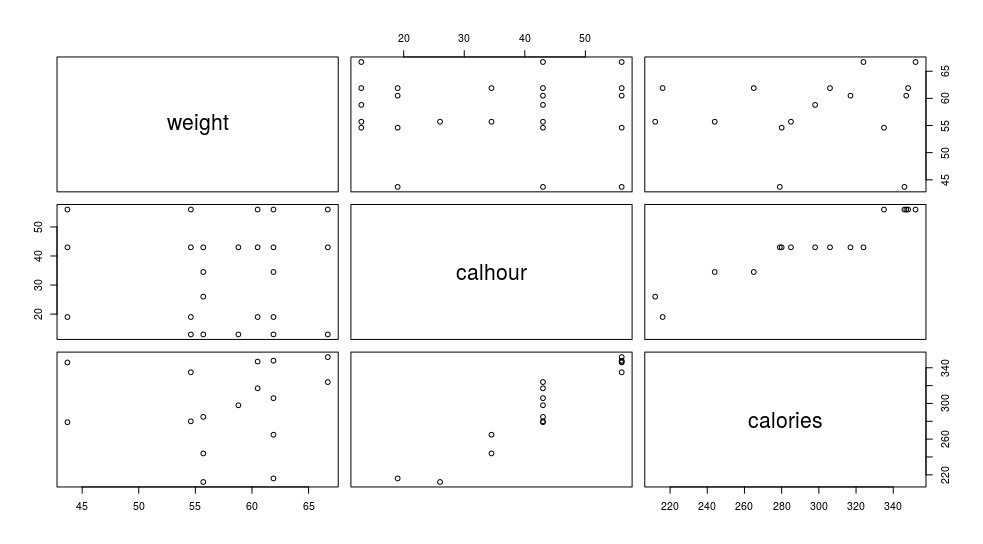
\includegraphics[scale=.55]{pairsplot.png}
    \caption{Pairs plot}
    \label{fig:pairs}
\end{figure}


In the following graphic (figure \ref{fig:xyplot}), we tried to
explore if there was an association between the weights (considered as
categorical variable this time) and a simple linear regression model
that explains the variability in calories spent by the single
covariate calhour. And indeed there seems to be an association, as the
lighter categories display steeper slopes than the heavier
categories. Note however that most categories only have 2
observations, hence the line fitting process is exact.

\begin{figure}[H]
    \centering
    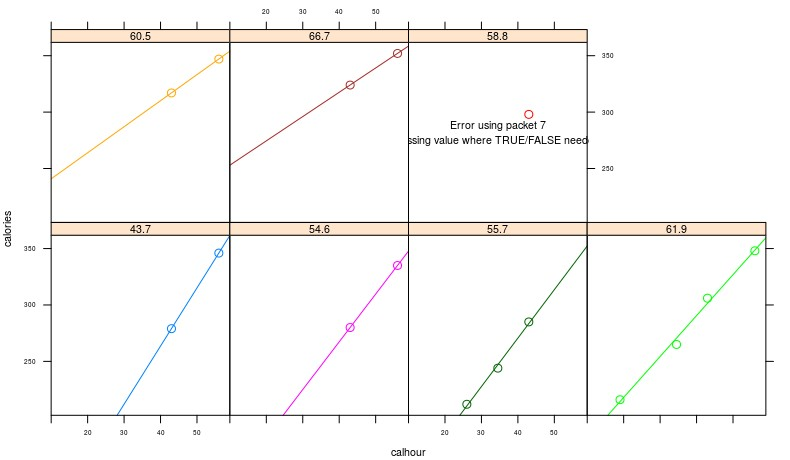
\includegraphics[scale=.6]{incomplete.jpg}
    \caption{xy plot of the linear regressions per categories}
    \label{fig:xyplot}
\end{figure}

To complete this exploratory analysis of the dataset, here is a table
of summary statistics for each of the variables taken separately. To
note is the number of NA values found in the calories column.

\begin{verbatim}
                  weight calhour calories
    nbr.val        24.00   24.00    16.00
    nbr.null        0.00    0.00     0.00
    nbr.na          0.00    0.00     8.00
    min            43.70   13.00   212.00
    max            66.70   56.00   352.00
    range          23.00   43.00   140.00
    sum          1381.00  817.00  4754.00
    median         58.80   38.75   302.00
    mean           57.54   34.04   297.12
    SE.mean         1.35    3.34    11.47
    CI.mean.0.95    2.78    6.91    24.44
    var            43.43  267.67  2103.85
    std.dev         6.59   16.36    45.87
    coef.var        0.11    0.48     0.15
\end{verbatim}


\begin{table}[H]
    \centering
    \begin{tabular}{l|l|l|l|}
    \cline{2-4}
                                   & weight & calhour & calories \\ \hline
    \multicolumn{1}{|l|}{weight}   & 1      & -0.026  & 0.111    \\ \hline
    \multicolumn{1}{|l|}{calhour}  & -0.026 & 1       & 0.951    \\ \hline
    \multicolumn{1}{|l|}{calories} & 0.111  & 0.951   & 1        \\ \hline
    \end{tabular}
    \caption{Correlation}    
\end{table}
\subsection{Missing data} \label{missing}

Below are visualizations of the measurements that are missing from the
dataset. From figure \ref{fig:aggrplot} we can deduce that all
participants in the study have been successfully weighed, but for one
third of the tests the amount of heat produced could not be
successfully measured. Of course calhour (the level of work to be done
by the participants) was fixed a priori and there are no missing
values for that variable.

\begin{figure}[H]
    \centering
    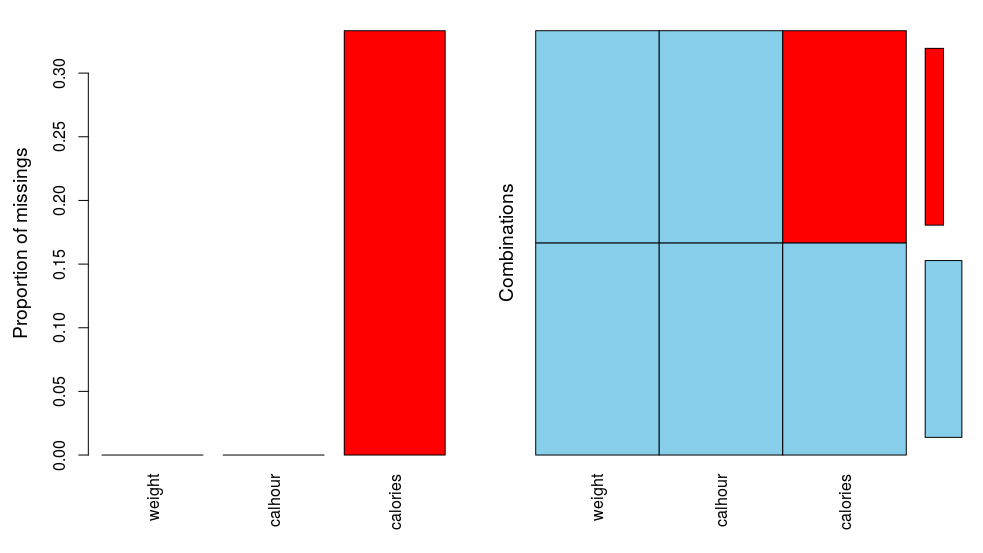
\includegraphics[scale=.4]{aggr.png}
    \caption{Aggr plot}
    \label{fig:aggrplot}
\end{figure}

Figure \ref{fig:barplotmiss} shows that the distribution of missing
data across the weight categories always remains close to its average
$\frac{1}{3}$-value. This means that the result of our analysis should
be valid across all weight categories in the study.

\begin{figure}[H]
    \centering
    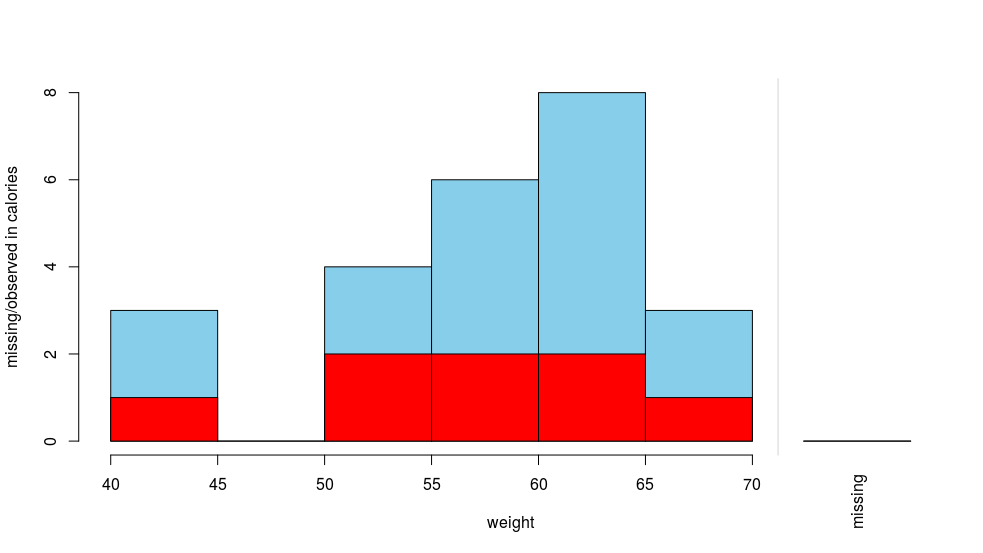
\includegraphics[scale=.6]{barplotmiss.png}
    \caption{Barplot missing data}
    \label{fig:barplotmiss}
\end{figure}

The same however cannot be said for the calhour variable. From the
boxplots on the left side in figure \ref{fig:marginplot} it is
apparent that all but one observation in the two lowest calhour
categories have missing values for the heat production calories. This
means our analysis might not be valid in the region of work level
values below 19 calhour.

\begin{figure}[H]
    \centering
    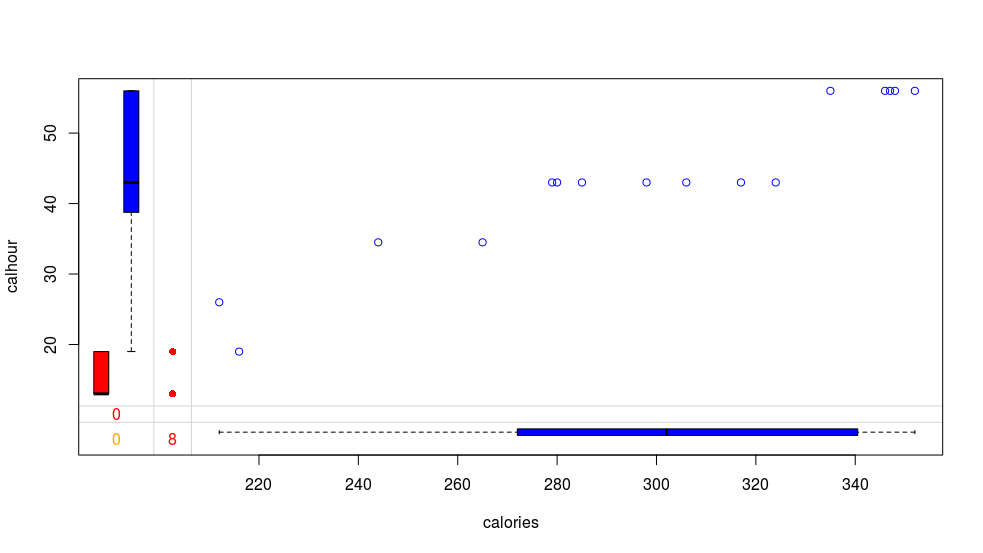
\includegraphics[scale=.5]{marginplot.png}
    \caption{Margin missing data}
    \label{fig:marginplot}
\end{figure}

\section{Complete case analysis}

From the exploration of the data we found out that there is a linear
relation between the calories and the calhour. For that reason, for
the complete case analysis we decided to try four different linear
models. The first model we tried was the one containing the weight,
the second model contained the calhour, the third model contained the
calhour and the weight and the fourth model contained the weight, the
calhour and an interaction term between those two variables.

Below, are the results of the analysis.

\begin{table}[H]
    \centering
    \begin{tabular}{l|l|l|l|l|}
    \cline{2-5}
                                         & lm1     & lm2    & lm3    & lm4    \\ \hline
    \multicolumn{1}{|l|}{Multiple R-squared} & 0.01241 & 0.9045 & 0.9436 & 0.9684 \\ \hline
    \multicolumn{1}{|l|}{F-statistic}        & 0.1759  & 132.6  & 108.8  & 122.5  \\ \hline
    \end{tabular}
    \caption{Models statistics comparisons}
\end{table}

Specifically, this is the summary output for the fourth model:

\begin{verbatim}
> summary(lm4)

Call:
lm(formula = calories ~ weight + calhour + I(weight * calhour))

Residuals:
   Min     1Q Median     3Q    Max 
-12.48  -5.70  -1.04   2.39  16.95 

Coefficients:
                    Estimate Std. Error t value Pr(>|t|)    
(Intercept)         -330.884    124.674   -2.65  0.02102 *  
weight                 7.728      2.106    3.67  0.00321 ** 
calhour               11.787      2.548    4.63  0.00058 ***
I(weight * calhour)   -0.132      0.043   -3.07  0.00977 ** 
---
Signif. codes:  0 ‘***’ 0.001 ‘**’ 0.01 ‘*’ 0.05 ‘.’ 0.1 ‘ ’ 1

Residual standard error: 9.1 on 12 degrees of freedom
  (8 observations deleted due to missingness)
Multiple R-squared:  0.968,	Adjusted R-squared:  0.96 
F-statistic:  123 on 3 and 12 DF,  p-value: 2.89e-09
\end{verbatim}

As we can see from the results the best model is the model containing
the interaction term, with multiple R-squared 0.9684. However, the
$R^2$ metrics is dangerous when evaluating different models because it
can only go up as you add more parameters and make the model more
complex.

\subsection{Comparison of models using AIC}

As mentioned above, the $R^2$ metric is not suitable for deciding
which model fits the data best. Such a test - in the case of nested
models - can be performed by calculating the AIC\footnote{Akaike
  Information Criterion $=-2 \log L+2p$, with $L$ the likelihood and
  $p$ the amount of parameters.} score for each model. It allows us to
take into account the goodness of fit of the model relative to the
complexity of the model. The R-output below appoints model 4 as the
best (lowest) one, using the AIC criterion:

\begin{verbatim}
> AIC(lm1)
172.598
> AIC(lm2)
135.2196
> AIC(lm3)
128.7919
> AIC(lm4)
121.5314
\end{verbatim}

\section{Missing data analysis}
We tried two different methods of dealing with missing values:
imputation and inverse probability weighting (IPW).Given that the
missing data was found systematically in the lower part of the calhour
surveyed, for example, no value for a calhour of 13 (out of 5 possible
measurements), and only 1 value for 19 (out of 4 possible
measurements), we inferred that the values were not missing at
random. Caution should hence be exerted when trying to investigate the
structure of the relationship in the lower part of our data. Note
however that because of the shear "physicality" of the experiments,
there is an expectation that for those lower values, lower amounts of
calories would also be measured.

\subsection{Multiple imputation analysis}
For multiple imputation we tried four different methods:
\begin{itemize}
    \item pmm(predictive mean matching)
    \item norm(Bayesian linear regression)
    \item norm.nob( linear regression non-Bayesian)
    \item sample(Random sampling from the observed data)
\end{itemize}

The best method were norm and norm.nob which follow the distribution
of the observed data with respect to the imputed data based on the
fact that most of the missing values for calhour were between 13-19
with just one observed value within the range. We then run the
imputation 5 and 100 times.

\subsubsection{Diagnostic checking in R}
\begin{verbatim}
Multiply imputed data set
Call:
mice(data = muscle, m = 100, method = c("", "", "norm.nob"))
Number of multiple imputations:  100
Missing cells per column:
  weight  calhour calories 
       0        0        8 
Imputation methods:
    weight    calhour   calories 
        ""         "" "norm.nob" 
VisitSequence:
calories 
       3 
PredictorMatrix:
         weight calhour calories
weight        0       0        0
calhour       0       0        0
calories      1       1        0
Random generator seed value:  NA 
\end{verbatim}


\begin{figure}[H]
    \centering
    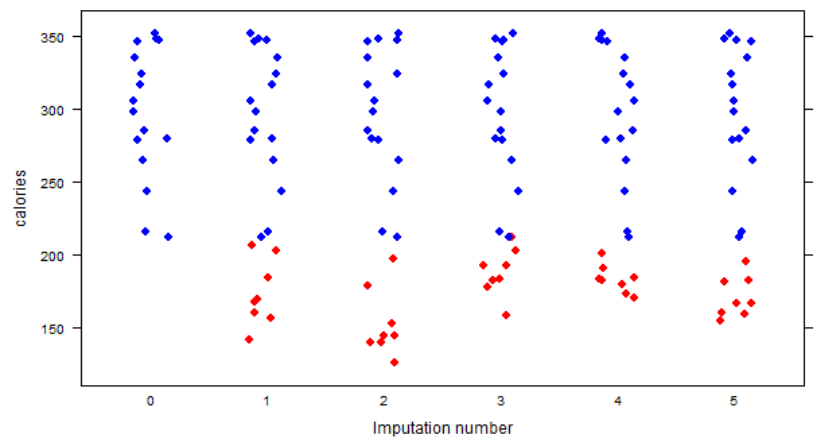
\includegraphics[scale=.5]{impu5.png}
    \caption{Imputation 5 rounds, the blue points indicates the
      observed data and the red points the imputed data.}
    \label{fig:imputation5}
\end{figure}


\begin{figure}[H]
    \centering
    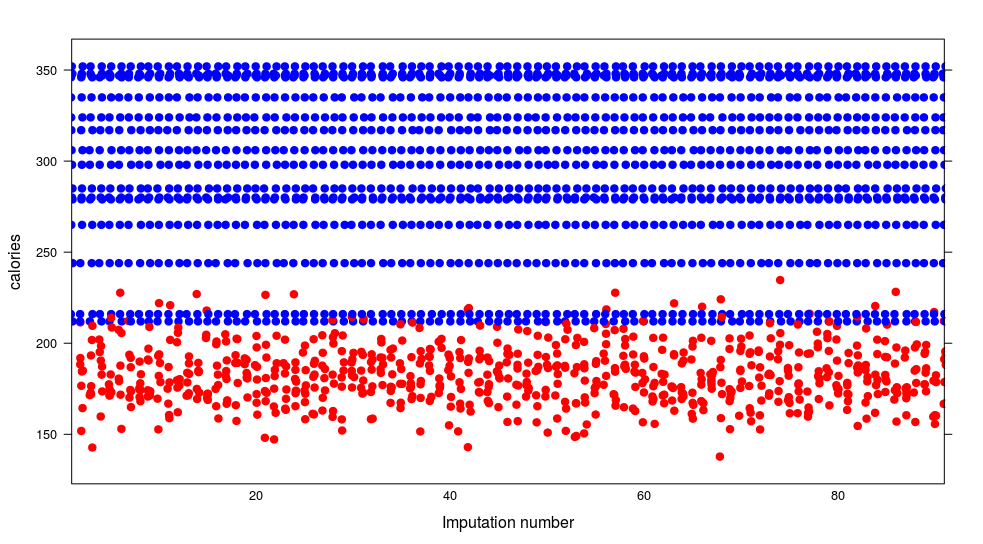
\includegraphics[scale=.5]{imputation100.png}
    \caption{Imputation 100 rounds, the blue points indicates the
      observed data and the red points the imputed data}
    \label{fig:imputation100}
\end{figure}

In figures \ref{fig:imputation5} and \ref{fig:imputation100} we can
see that most of the points cluster around 150-200. Given our
assumption mentioned above concerning the "physicality" of this study,
we consider that the imputed data are plausible.

\subsubsection{Analysis the imputed data sets}
Since the complete-data analysis of interest is a linear regression of
calories on weight and calhour plus the interaction term. As such, we
use the function with(), which is a wrapper function that applies the
complete data model to each of the imputed data sets.

\begin{verbatim}
                            est          se          t        df
(Intercept)         -9.41464218 74.87464828 -0.1257387  8.575972
weight               2.29149915  1.28545302  1.7826394  8.578415
calhour              5.39761221  1.65453674  3.2623103 10.407747
I(weight * calhour) -0.02405517  0.02839728 -0.8470941 10.406311

                       Pr(>|t|)         lo 95        hi 95 nmis       fmi
(Intercept)         0.902836870 -180.07810098 161.24881663   NA 0.6022167
weight              0.109965962   -0.63832841   5.22132670    0 0.6020881
calhour             0.008114754    1.73055823   9.06466619    0 0.5059371
I(weight * calhour) 0.415999085   -0.08699498   0.03888464   NA 0.5060124

                       lambda
(Intercept)         0.5191372
weight              0.5190029
calhour             0.4193183
I(weight * calhour) 0.4193959
\end{verbatim}

\subsection{IPW analysis}
Inverse probability weighting recovers consistent estimates when data
are missing at random. Two things are needed for IPW methods:
\begin{itemize}
    \item A response model relating the response to the predictor variables;
    \item An absence model for the probability of missing observations.
\end{itemize}
The former is usually a multivariate regression; it is part of the
analysis we would do if the data were fully observed.

The latter is usually a logistic regression that provides a value for
each individual in the dataset, which is an estimate of the
probability of this individual having a missing value for the response
variable, based on the values of the predictor variables.

The first step for calculating the absence model is to create a new
indicator variable $r$ with $r=0$ when calories is missing and $r=1$
when calories are observed.
\begin{verbatim}
> head(muscle.missing,5)
    weight  calhour calories    r
1    43.7    19.0       NA      0
2    43.7    43.0      279      1
3    43.7    56.0      346      1
4    54.6    13.0       NA      0
5    54.6    19.0       NA      0
\end{verbatim}

Based on these values we then fit the absence model, which is a
logistic model for $r$.
\begin{verbatim}
> summary(muscle.ipw.glm)

Call:
glm(formula = r ~ weight + calhour, family = binomial, data = muscle.missing, 
    control = list(maxit = 500))

Deviance Residuals: 
       Min          1Q      Median          3Q         Max  
-1.354e-05  -2.110e-08   2.110e-08   2.110e-08   1.388e-05  

Coefficients:
              Estimate Std. Error z value Pr(>|z|)
(Intercept)   -2671.19 4988005.76  -0.001        1
weight           32.98   63223.78   0.001        1
calhour          34.35   62815.06   0.001        1

(Dispersion parameter for binomial family taken to be 1)

    Null deviance: 3.0553e+01  on 23  degrees of freedom
Residual deviance: 4.1288e-10  on 21  degrees of freedom
AIC: 6

Number of Fisher Scoring iterations: 29
\end{verbatim}

Now our next step would be to calculate the inverse probabilities
(weights $w_i$) based on the logistic regression model above, and use
them to modify the contributions of each individual $i$ in the reponse
model. They can be calculated as
\[w_i=(\text{fitted probability from the absence model})^{-1}\]
and then used to refit the response model. However, during the
calculation (result shown below) we run into a problem:
\begin{verbatim}
> head(muscle.missing,5)
    weight  calhour calories  r         w
1    43.7    19.0       NA    0    4.503600e+15
2    43.7    43.0      279    1    1.000000e+00
3    43.7    56.0      346    1    1.000000e+00
4    54.6    13.0       NA    0    4.503600e+15
5    54.6    19.0       NA    0    4.503600e+15
\end{verbatim}
These values for the weights are either equal to $1$ or extremely
large. This is the result of a warning R gives you when computing the
absence model:
\begin{verbatim}
glm.fit: fitted probabilities numerically 0 or 1 occurred
\end{verbatim}
This is because in the lowest calhour category there is not a single
observed value for calories (easily seen in figure
\ref{fig:marginplot}). The glm function used in fitting the absence
model detects this and therefore the fitted model will return a
probability that is exactly zero for every observation in the
calhour$=13$ category. This results in an infinite-valued weight,
which might explain the enormous values in the $w$ column above. We
expect something similar is happening to the calhour=$19$ category,
and we can thereby conclude the IPW analysis is unfit for this
dataset.

\section{Comparative analysis and Conclusion}
To compare the two different ways of analyzing the data we look at
table \ref{tab:comparison}. Clearly the models are not in agreement,
since the estimates of coefficients in one model $Estimate_1$ fall
outside the range determined by the estimates and standard error of
the other model $Estimate_2 \pm Std Error$. This could be due to the
nonlinearity (in the resulting hypersurface) introduced by using the
interaction term. When performing the same comparison of models using
this time lm3, which fits a hyperplane through the data, the
parameters are much closer and within range of std error. The
flexibility of the hypersurface generated in lm4 results in higher
variance outside the region of the original complete data points.

\begin{table}[H]
\centering
\begin{tabular}{l|l|l|l|l|}
\cline{2-5}
                                          & \multicolumn{2}{c|}{Imputed data case}                         & \multicolumn{2}{c|}{Complete case}                             \\ \hline
\multicolumn{1}{|c|}{Coefficient}         & \multicolumn{1}{c|}{Estimate} & \multicolumn{1}{c|}{Std Error} & \multicolumn{1}{c|}{Estimate} & \multicolumn{1}{c|}{Std Error} \\ \hline
\multicolumn{1}{|l|}{(Intercept)}         & -9.41464218                   & 74.87464828                    & -330.884                      & 124.674                        \\ \hline
\multicolumn{1}{|l|}{weight}              & 2.29149915                    & 1.28545302                     & 7.728                         & 2.106                          \\ \hline
\multicolumn{1}{|l|}{calhour}             & 5.39761221                    & 1.65453674                     & 11.787                        & 2.548                          \\ \hline
\multicolumn{1}{|l|}{I(weight * calhour)} & -0.02405517                   & 0.02839728                     & -0.132                        & 0.043                          \\ \hline
\end{tabular}
\caption{Comparison between coefficient values of the imputed data case and the complete case.}
\label{tab:comparison}
\end{table}

However, what the models do agree about are the signs of the
coefficients. The intercept is probably negative, and both weight and
the amount of work done by the individuals have a positive effect on
the amount of heat produced. The latter two statements seem logical,
since heavier people have on average more volume to produce heat with,
and and increasingly heavy workouts also make you produce an
increasing amount of heat. The standard errors for both cases are
quite large, with the ones of the complete case being relatively lower
but higher in absolute value.

In general, we conclude that due to the systematic structure of
missing data in the lower part of the calhour, and the very low amount
of observations in our original dataset (only 16 points), we cannot
ascertain whether the linear trend observed in the upperpart of the
dataset can be extended to the missing part, and that modelling
activity in our case cannot replace a more thourough experimental
investigation.


\bibliographystyle{ieeetr} 
\bibliography{bib-db}

\newpage

\appendix
\section{Supplementary information}
\subsection{Clustering}
Figure \ref{fig:spaghettiplot} is a profile plot of the data, which
was first centered for ease of comparison. The calhour clustering can
be ignored because they are just the categories which have been
defined in advance. The clustering in weight is just due to the same
person performing the test at multiple work levels. No clustering is
observed for the amount of heat produced. A remarkable thing though is
that clearly for the lowest work level, not a single successful
measurement of heat production was done (all lines going through that
lowest point of calhour end in that point). The missing data is
discussed in more detail in section \ref{missing}.
\begin{figure}[H]
    \centering
    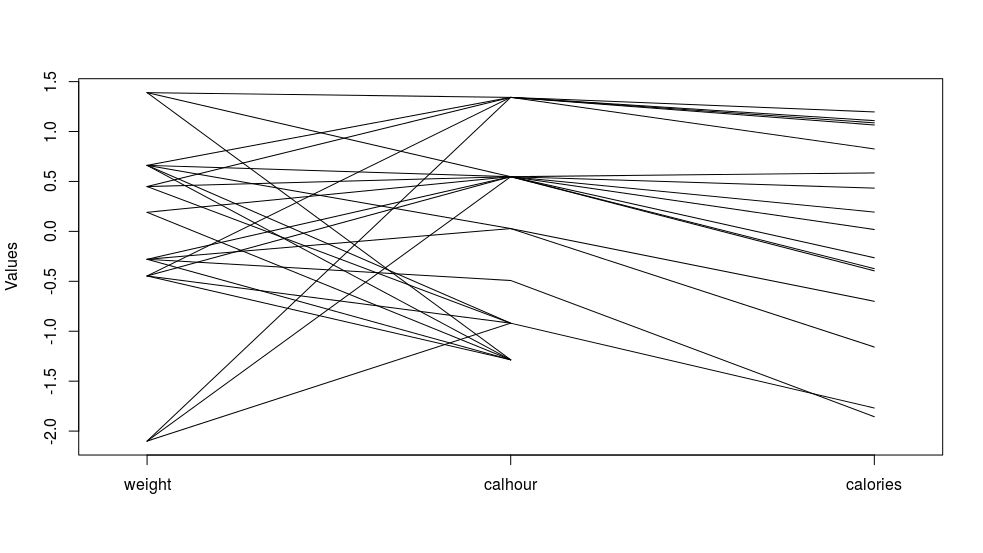
\includegraphics[scale=.5]{spaghettiplot.png}
    \caption{Spaghetti plot}
    \label{fig:spaghettiplot}
\end{figure}

\subsection{3D Scatterplot}
One of the first attempts at understanding the structure of our data
was to use a scatterplot. Given that we have 3 variables in total, we
explored using a rotable 3D scatterplot and found a very strong linear
trend in the data, as illustrated in figure \ref{fig:3DScatterplot}
where the different clusters of weights have been colored:
\begin{figure}[H]
    \centering
    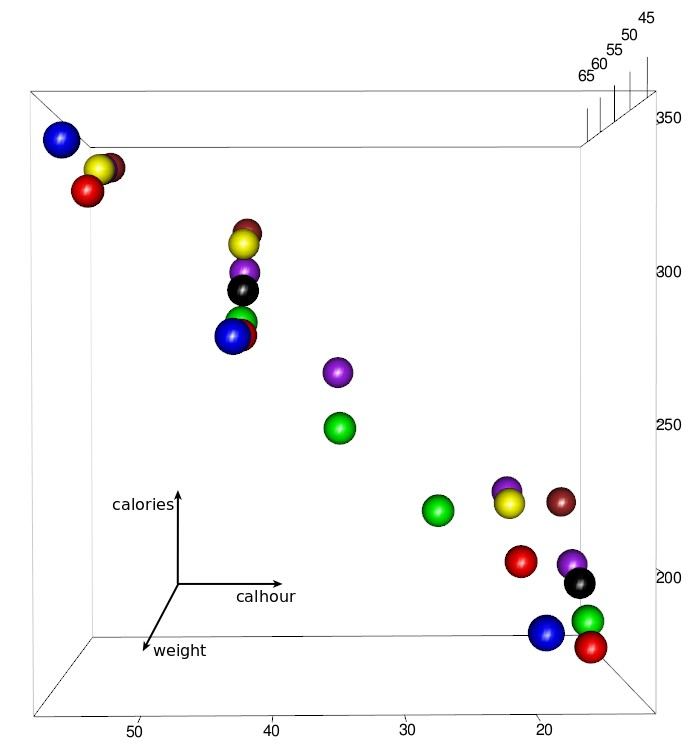
\includegraphics[scale=.4]{3DScatterplot.jpg}
    \caption{3D Scatterplot oriented to visualise the linear trend}
    \label{fig:3DScatterplot}
\end{figure}

\subsection{Log-likelihood comparison}
To get a sense of how significant the difference between lm4 and lm3
is, we can look at the difference of their log-likelihoods. This
criterion however does not take the amount of parameters into account,
so in a sense it provides less information than the AIC. However we
can assign a p-value to this test, which may further boost or rather
undermine confidence in the previous finding that lm4 is the best
model.

Multiplied by two, the value follows a $\chi^2$-distribution with one
(the difference in amount of parameters between the two models) degree
of freedom:
\begin{verbatim}
> lL3 <- logLik(lm3, REML = FALSE)
> lL4 <- logLik(lm4, REML = FALSE)
> lL3
'log Lik.' -60.39594 (df=4)
> lL4
'log Lik.' -55.76572 (df=5)
> 2*(lL4-lL3)
'log Lik.' 9.26043 (df=5)
\end{verbatim}
The resulting value $9.26043$ is larger than the 0.01-level value of
the corresponding $\chi^2$-distribution, which is valued at
$6.63$. This means we can say lm4 is more likely than lm1 on a p=0.01
significance level, but not taking the amount of parameters into
account.

\end{document}
